\section{PMMA without doping}
\subsection*{Material ID: Thickness: 100}
\textbf{Constante Dieléctrica ($\epsilon_{total}$):} 2.52 \\[0.5em]
\begin{table}[h!]
\centering
\begin{tabular}{lcc}
\toprule
\textbf{Métrica} & \textbf{Lámina (Plate)} & \textbf{Cilindros (Rod)} \\
\midrule
Bandgaps ($k_x$) & Ninguno & Ninguno \\
Resonancias ($k_x$) & 36 & 36 \\
\midrule
Bandgaps (Rotación) & Ninguno & Ninguno \\
Resonancias (Rotación) & 33 & 33 \\
\bottomrule
\end{tabular}
\end{table}
\begin{figure}[H]
\centering
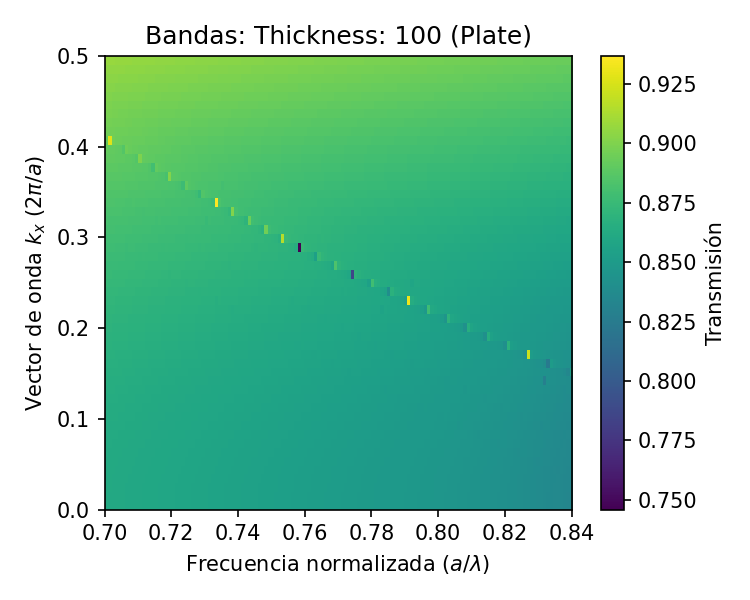
\includegraphics[width=0.48\textwidth]{figures/Thickness: 100_plate.png}
\hfill
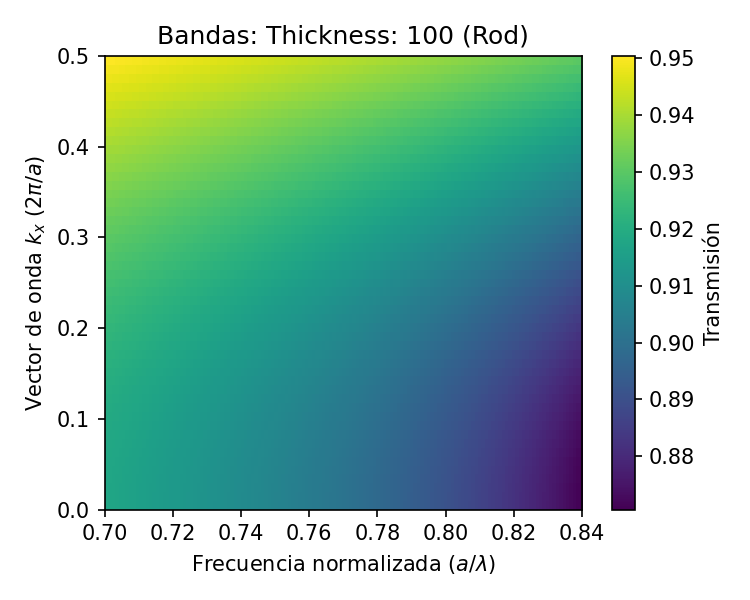
\includegraphics[width=0.48\textwidth]{figures/Thickness: 100_rod.png}
\caption{Estructuras de bandas fotónicas ($k_x$) para Thickness: 100. Izquierda: Lámina. Derecha: Cilindros.}
\end{figure}
\vspace{1em}
\begin{figure}[H]
\centering
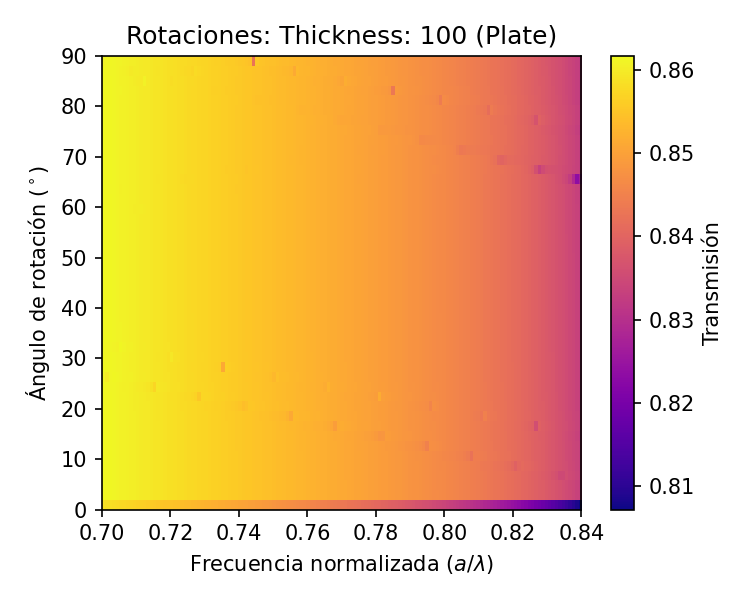
\includegraphics[width=0.48\textwidth]{figures/Thickness: 100_plate_rangle.png}
\hfill
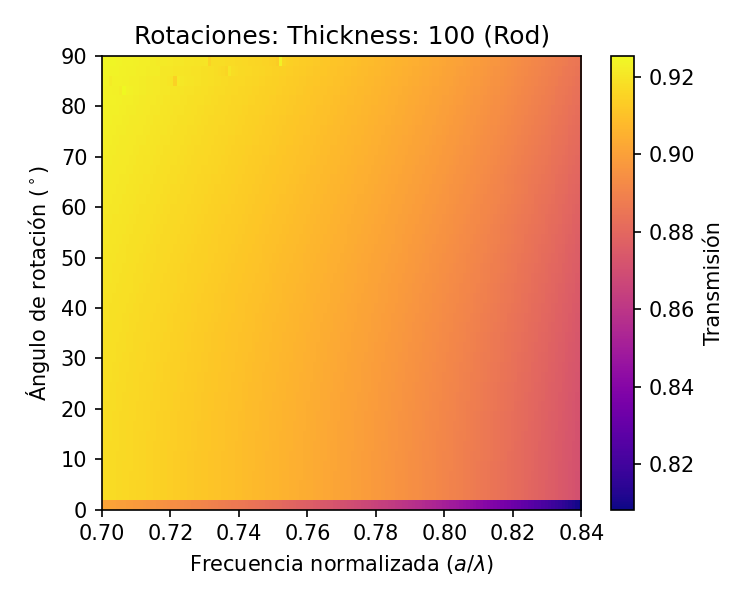
\includegraphics[width=0.48\textwidth]{figures/Thickness: 100_rod_rangle.png}
\caption{Mapas de transmisión por rotación (twist) para Thickness: 100. Izquierda: Lámina. Derecha: Cilindros.}
\end{figure}
\vspace{1em}
\hrule
\vspace{1em}
\subsection*{Material ID: Thickness: 150}
\textbf{Constante Dieléctrica ($\epsilon_{total}$):} 2.53 \\[0.5em]
\begin{table}[h!]
\centering
\begin{tabular}{lcc}
\toprule
\textbf{Métrica} & \textbf{Lámina (Plate)} & \textbf{Cilindros (Rod)} \\
\midrule
Bandgaps ($k_x$) & Ninguno & Ninguno \\
Resonancias ($k_x$) & 36 & 36 \\
\midrule
Bandgaps (Rotación) & Ninguno & Ninguno \\
Resonancias (Rotación) & 33 & 33 \\
\bottomrule
\end{tabular}
\end{table}
\begin{figure}[H]
\centering
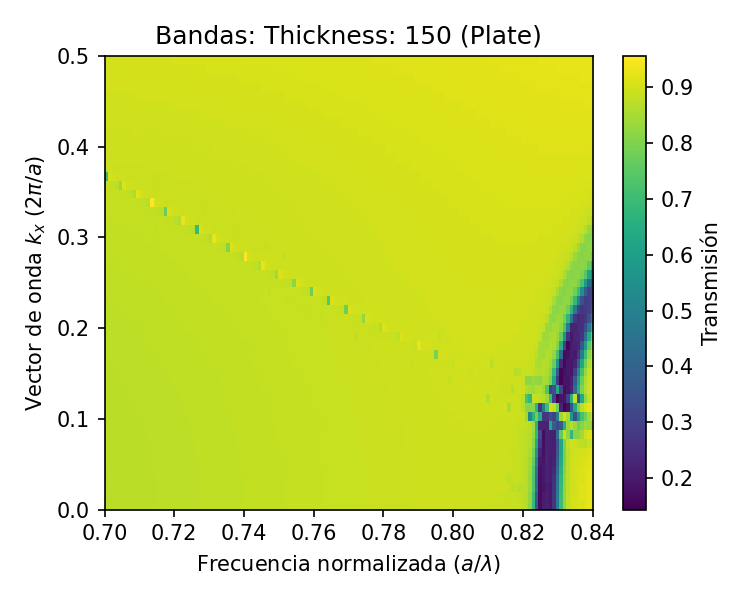
\includegraphics[width=0.48\textwidth]{figures/Thickness: 150_plate.png}
\hfill
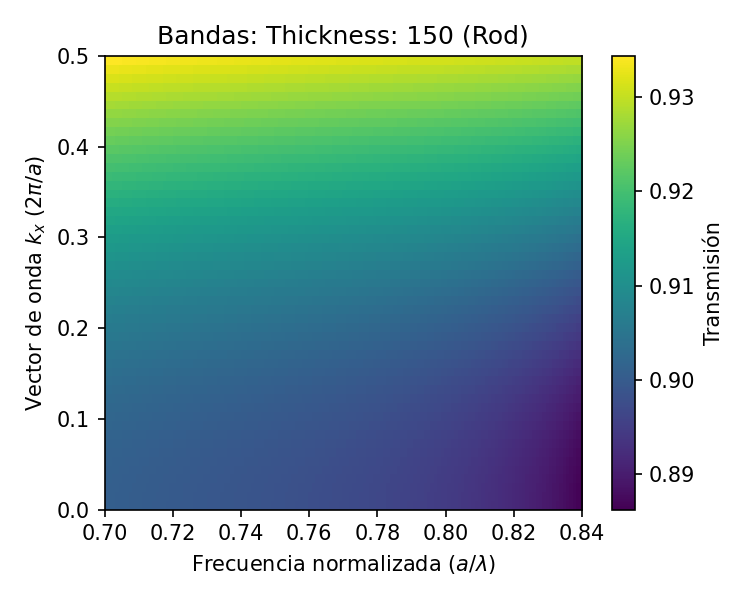
\includegraphics[width=0.48\textwidth]{figures/Thickness: 150_rod.png}
\caption{Estructuras de bandas fotónicas ($k_x$) para Thickness: 150. Izquierda: Lámina. Derecha: Cilindros.}
\end{figure}
\vspace{1em}
\begin{figure}[H]
\centering
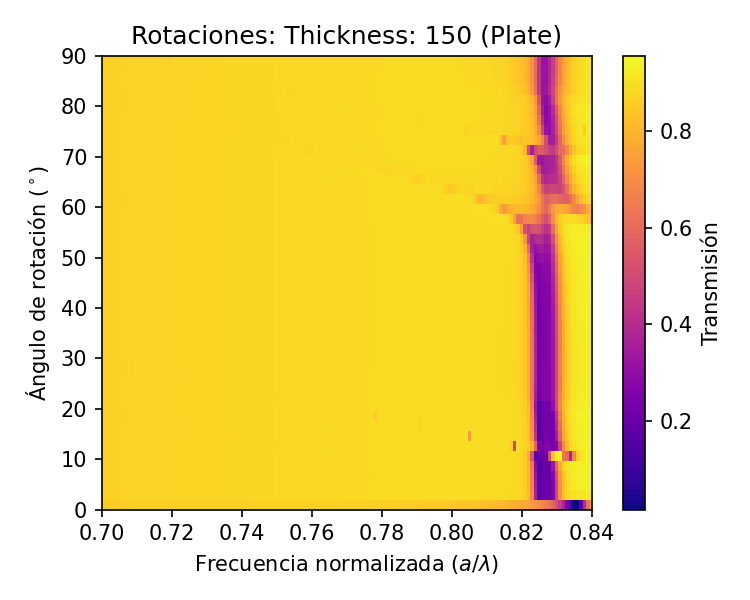
\includegraphics[width=0.48\textwidth]{figures/Thickness: 150_plate_rangle.png}
\hfill
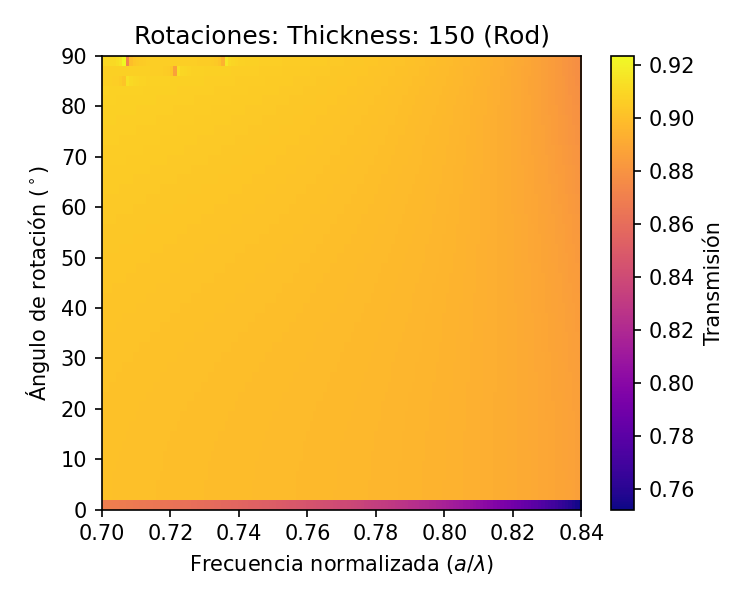
\includegraphics[width=0.48\textwidth]{figures/Thickness: 150_rod_rangle.png}
\caption{Mapas de transmisión por rotación (twist) para Thickness: 150. Izquierda: Lámina. Derecha: Cilindros.}
\end{figure}
\vspace{1em}
\hrule
\vspace{1em}
\subsection*{Material ID: Thickness: 200}
\textbf{Constante Dieléctrica ($\epsilon_{total}$):} 2.47 \\[0.5em]
\begin{table}[h!]
\centering
\begin{tabular}{lcc}
\toprule
\textbf{Métrica} & \textbf{Lámina (Plate)} & \textbf{Cilindros (Rod)} \\
\midrule
Bandgaps ($k_x$) & Ninguno & Ninguno \\
Resonancias ($k_x$) & 36 & 36 \\
\midrule
Bandgaps (Rotación) & Ninguno & Ninguno \\
Resonancias (Rotación) & 33 & 33 \\
\bottomrule
\end{tabular}
\end{table}
\begin{figure}[H]
\centering
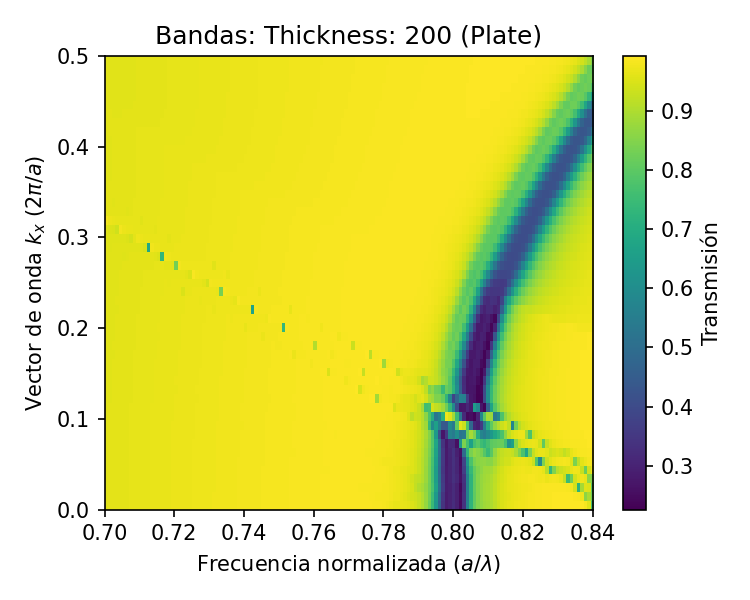
\includegraphics[width=0.48\textwidth]{figures/Thickness: 200_plate.png}
\hfill
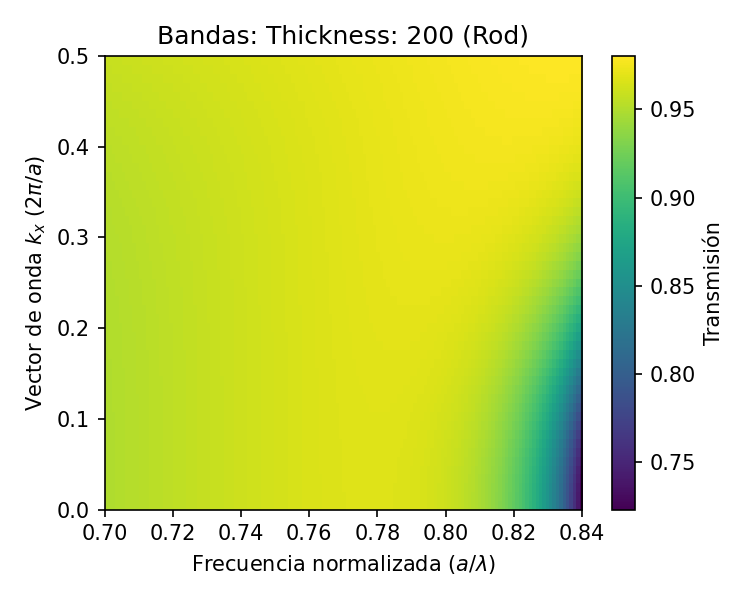
\includegraphics[width=0.48\textwidth]{figures/Thickness: 200_rod.png}
\caption{Estructuras de bandas fotónicas ($k_x$) para Thickness: 200. Izquierda: Lámina. Derecha: Cilindros.}
\end{figure}
\vspace{1em}
\begin{figure}[H]
\centering
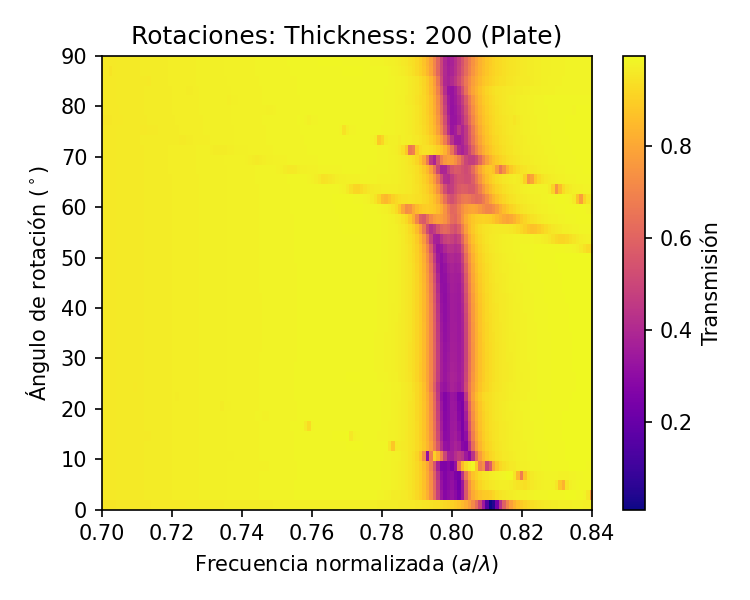
\includegraphics[width=0.48\textwidth]{figures/Thickness: 200_plate_rangle.png}
\hfill
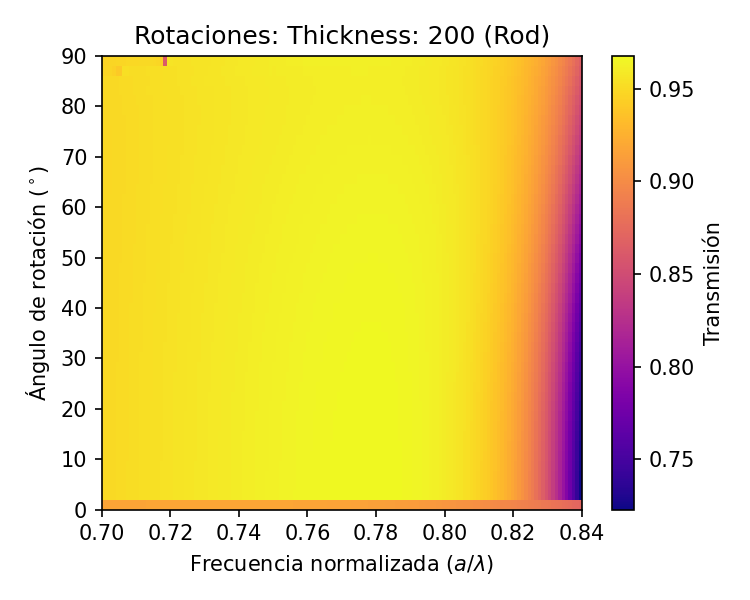
\includegraphics[width=0.48\textwidth]{figures/Thickness: 200_rod_rangle.png}
\caption{Mapas de transmisión por rotación (twist) para Thickness: 200. Izquierda: Lámina. Derecha: Cilindros.}
\end{figure}
\vspace{1em}
\hrule
\vspace{1em}
\subsection*{Material ID: Thickness: 60}
\textbf{Constante Dieléctrica ($\epsilon_{total}$):} 2.67 \\[0.5em]
\begin{table}[h!]
\centering
\begin{tabular}{lcc}
\toprule
\textbf{Métrica} & \textbf{Lámina (Plate)} & \textbf{Cilindros (Rod)} \\
\midrule
Bandgaps ($k_x$) & Ninguno & Ninguno \\
Resonancias ($k_x$) & 36 & 36 \\
\midrule
Bandgaps (Rotación) & Ninguno & Ninguno \\
Resonancias (Rotación) & 33 & 33 \\
\bottomrule
\end{tabular}
\end{table}
\begin{figure}[H]
\centering
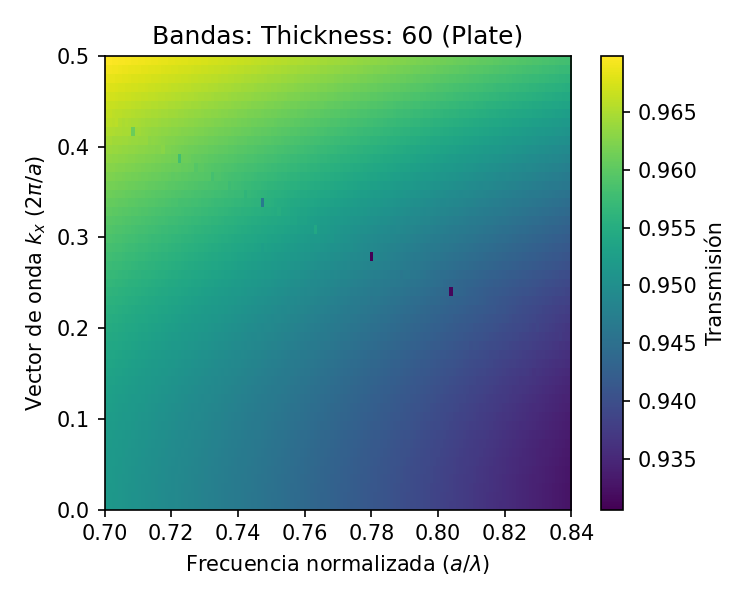
\includegraphics[width=0.48\textwidth]{figures/Thickness: 60_plate.png}
\hfill
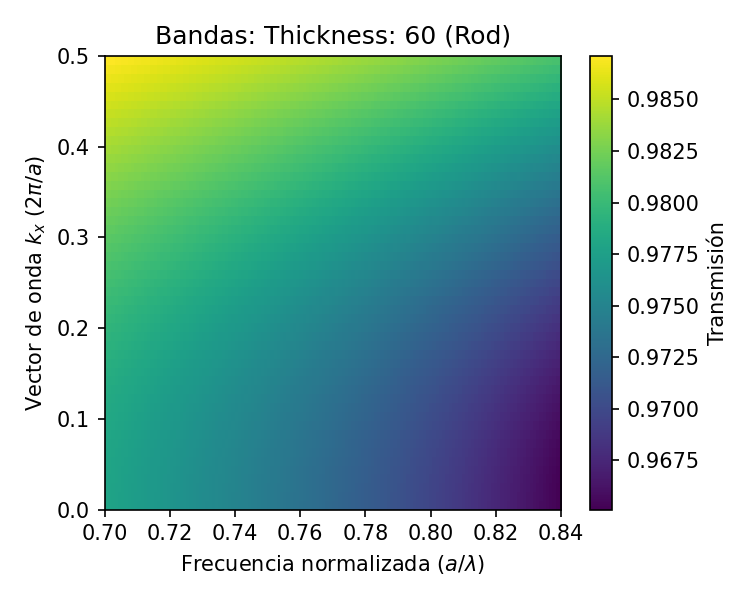
\includegraphics[width=0.48\textwidth]{figures/Thickness: 60_rod.png}
\caption{Estructuras de bandas fotónicas ($k_x$) para Thickness: 60. Izquierda: Lámina. Derecha: Cilindros.}
\end{figure}
\vspace{1em}
\begin{figure}[H]
\centering
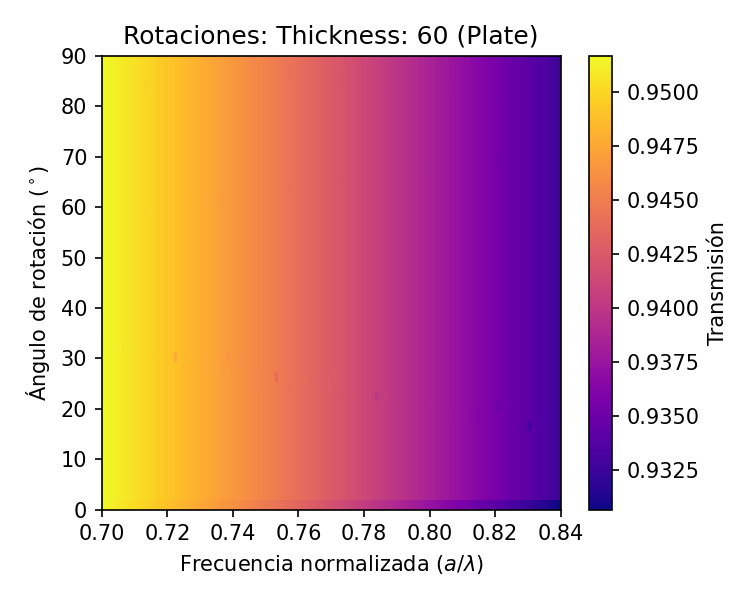
\includegraphics[width=0.48\textwidth]{figures/Thickness: 60_plate_rangle.png}
\hfill
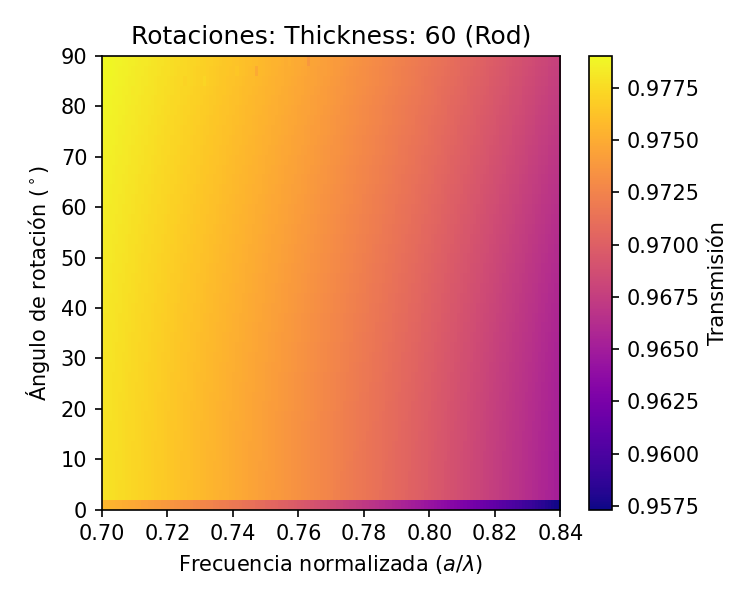
\includegraphics[width=0.48\textwidth]{figures/Thickness: 60_rod_rangle.png}
\caption{Mapas de transmisión por rotación (twist) para Thickness: 60. Izquierda: Lámina. Derecha: Cilindros.}
\end{figure}
\vspace{1em}
\hrule
\vspace{1em}
\clearpage